Die S0-Schnitstelle wird nach \textit{DIN EN 62053-31 definiert} und in der Geb�udeautomatisierung
verwendet. Die Schnittstelle wird in Elektrizit�tsz�hlern eingebaut. Mit
Impulseinrichtungen wie die S0-Schnittstelle werden Impulse, die der aktuell verbrauchten
Energiemenge entsprechen, an den Empf�nger �bertragen \cite[][][s0norm S.4].

\begin{figure}[htbp]
	\caption{S0-Schnitstelle in Stromz�hlern}
	\label{fig:S0Schnitstelle in Stromz�hlern}
	\centering
		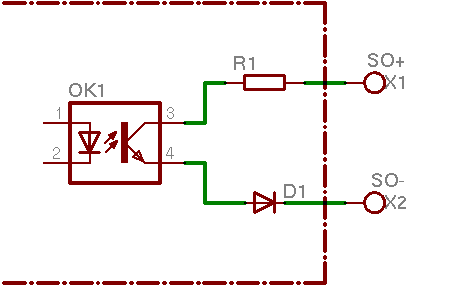
\includegraphics[width=0.40\textwidth]{Bilder/S0.png}
\end{figure}

Die Impulseinrichtungen geben eine bestimme Anzahl von Impulsen pro Wattstunde.
Dabei gibt es zwei Arten bzw. Klassen von Impulsausg�ngen [s0 norm S.5]:

\begin{description}
	\item[Impulsausgang der Klasse A:] �bertragung �ber gr��ere Entfernungen;
	\item[Impulsausgang der Klasse B:] geringe Entfernung und geringer Energieverbrauch
\end{description}

Dabei kann die Schnittstelle sowohl im Stromz�hler als auch im Gas- oder Wasserz�hler
eingesetzt werden. Bei der �bertragung von Messwerten wird f�r jedes
verbrauchtes Watt pro Stunde (Wph) ein gewichteter Impuls �bertragen. Die Gewichtung
des Impulses ist von Z�hler zu Z�hler unterschiedlich [vgl. S0S]. F�r die zwei
Arten bzw. Klassen von Impulsausg�ngen sind den Impulsen verschiedene Grenzen
gesetzt:

\begin{table}[!htbp]
	\centering
	\caption{S0-Schnitstelle in Stromz�hlern}
	\label{tab:S0SchnitstelleInStromz�hlern}
	
		\begin{tabular}{|c|c|c|}
				\hline
				
				Parameter & \multicolumn{1}{c|}{\begin{tabular}[c]{@{}c@{}}Impulseinrichtung\\ der Klasse A\end{tabular}} & \multicolumn{1}{c|}{\begin{tabular}[c]{@{}c@{}}Impulseinrichtung\\ der Klasse B\end{tabular}} \\ \hline
				Maximale Spannung U$_{max}$    & 27 V DC 												& 15 V DC		\\ \hline
				Maximaler Strom im EIN-Zustand & 27 mA   												& 15 mA 		\\ \hline
				Minimaler Strom im EIN-Zustand & 10 V DC 												& 2 V DC 		\\ \hline
				Maximaler Strom im Aus-Zustand & 2 V DC  												& 0,15 V DC \\ \hline
		\end{tabular}
		\\\quelle{asd}
\end{table}

Die Impulse k�nnen zwei Zust�nde haben: High- bzw. Ein- Zustand und Low- bzw.-
Aus-Zustand, f�r zwei aufeinanderfolgende Impulse.

\begin{figure}[!htbp]
	\caption{S0-Impulsform}
	\label{fig:S0_Impulsform}
	\centering
		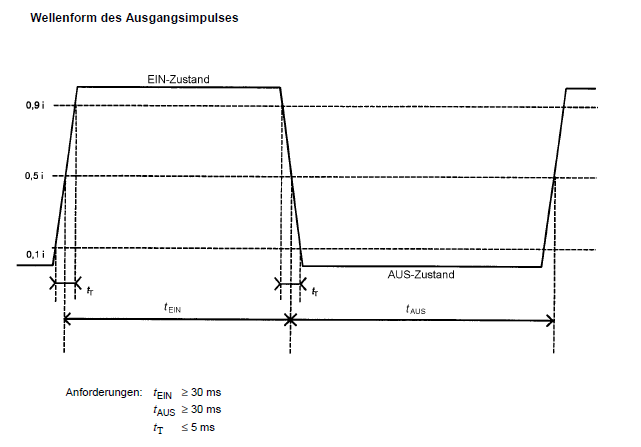
\includegraphics[width=0.70\textwidth]{Bilder/S0_Impulsform.png}
		\quelle{[asd]}
\end{figure}

F�r die Zust�nde sind die folgenden Impulsl�ngen definiert:
\begin{description}
	\item[] Ein Impuls, im \underline{High- bzw. Ein- Zustand}, ist mit t$_{EIN}\geq$ 30 ms, also gr��er gleich 30 ms definiert und der
	\item[] \underline{Aus- bzw- Low-Zustand}, f�r die Zeit zwischen zwei aufeinanderfolgenden Impulsen, mit t$_{AUS}$ $\geq$ 30 ms, also gr��er gleich 30 ms
\end{description}
Dabei muss die �bergangszeit der Anstiegs- oder Abfallzeit zwischen den einzelnen Zust�nden, also der Zustandswechsel 5 ms sein.